% Biên dịch bằng XeLaTeX (Overleaf: Menu > Compiler > XeLaTeX).
% Hoặc chạy: tectonic bao-cao-brewlite.tex
\documentclass[12pt,a4paper]{article}
\usepackage[margin=2.3cm,headheight=16pt]{geometry}
\usepackage{fontspec}
\setmainfont{texgyretermes-regular.otf}[BoldFont=texgyretermes-bold.otf,ItalicFont=texgyretermes-italic.otf,BoldItalicFont=texgyretermes-bolditalic.otf]
\setsansfont{texgyreheros-regular.otf}[BoldFont=texgyreheros-bold.otf,ItalicFont=texgyreheros-italic.otf,BoldItalicFont=texgyreheros-bolditalic.otf]
\setmonofont{lmmono10-regular.otf}[Scale=0.82]
\usepackage{polyglossia}
\setdefaultlanguage{vietnamese}
\usepackage{graphicx,booktabs,tabularx,longtable,array,multirow,amssymb}
\usepackage[table]{xcolor}
\usepackage{tikz}
\usetikzlibrary{arrows.meta,positioning,shapes.geometric,fit,backgrounds,calc}
\usepackage{enumitem,float,caption,pdflscape,fancyhdr,setspace,titlesec}
\usepackage[unicode,hidelinks]{hyperref}
\usepackage{xurl}
\definecolor{muc}{HTML}{173F35}
\definecolor{nhat}{HTML}{EDF4F0}
\definecolor{vien}{HTML}{C9D8D1}
\definecolor{chu}{HTML}{26352E}
\color{chu}
\hypersetup{pdftitle={BrewLite - Assignment 2: Từ yêu cầu đến triển khai},pdfauthor={Nhóm BrewLite}}
\setlength{\parindent}{1.0cm}
\setlength{\parskip}{4pt}
\setlength{\emergencystretch}{4em}
\setstretch{1.15}
\setlist{nosep,leftmargin=1.6em,topsep=4pt}
\setcounter{secnumdepth}{3}
\setcounter{tocdepth}{2}
\renewcommand{\arraystretch}{1.18}
\newcolumntype{Y}{>{\raggedright\arraybackslash}X}
\newcolumntype{P}[1]{>{\raggedright\arraybackslash}p{#1}}
\captionsetup{font=small,labelfont=bf,skip=8pt}
\titleformat{\section}{\Large\bfseries\color{muc}}{\thesection.}{0.5em}{}
\titleformat{\subsection}{\large\bfseries\color{muc}}{\thesubsection.}{0.5em}{}
\titleformat{\subsubsection}{\normalsize\bfseries}{\thesubsubsection.}{0.5em}{}
\pagestyle{fancy}
\fancyhf{}
\fancyhead[L]{\small BREWLITE | ASSIGNMENT 2}
\fancyhead[R]{\small Công nghệ Phần mềm}
\fancyfoot[C]{\thepage}
\renewcommand{\headrulewidth}{0.4pt}
\newcommand{\tep}[1]{\nolinkurl{#1}}
\newcommand{\canbosung}[1]{\textit{[Cần bổ sung: #1]}}
\newcommand{\ghichu}[1]{\begin{quote}\small\textbf{Ghi chú minh chứng.} #1\end{quote}}
\newcommand{\TenNhom}{\canbosung{tên hoặc số nhóm}}
\newcommand{\LopHoc}{\canbosung{lớp học phần}}
\newcommand{\GiangVien}{\canbosung{họ tên giảng viên}}
\tikzset{
  hop/.style={draw=vien,fill=nhat,rounded corners=3pt,align=center,font=\small,inner sep=7pt},
  tacvu/.style={hop,text width=3.3cm,minimum height=0.8cm},
  usecase/.style={ellipse,draw=muc,fill=nhat,align=center,text width=3.2cm,font=\small,minimum height=0.9cm},
  mui/.style={-{Latex[length=2mm]},draw=muc,line width=0.65pt},
  nhan/.style={font=\scriptsize,fill=white,inner sep=2pt,align=center},
  quyetdinh/.style={diamond,aspect=2.2,draw=muc,fill=nhat,font=\small,align=center,inner sep=2pt,text width=2.2cm},
  lop/.style={draw=muc,fill=white,align=left,font=\small,text width=4.1cm,inner sep=7pt},
}

\begin{document}
\hypersetup{pageanchor=false}
\begin{titlepage}
\centering
{\large\bfseries TRƯỜNG ĐẠI HỌC SÀI GÒN\par}
{\large KHOA CÔNG NGHỆ THÔNG TIN\par}
\vspace{0.7cm}
\rule{0.7\textwidth}{0.6pt}\par
\vspace{1.1cm}
{\Large\bfseries BÁO CÁO BÀI TẬP LỚN\par}
\vspace{0.4cm}
{\Huge\bfseries\color{muc} BREWLITE\par}
\vspace{0.35cm}
{\LARGE Assignment 2\par}
\vspace{0.35cm}
{\Large TỪ YÊU CẦU ĐẾN TRIỂN KHAI\par}
\vspace{0.8cm}
\begin{tabular}{ll}
Môn học: & Công nghệ Phần mềm\\
Công nghệ: & Next.js, NestJS, PostgreSQL, Docker\\
Học kỳ: & I - Năm học 2026--2027\\
Giảng viên: & \GiangVien\\
Lớp học phần: & \LopHoc\\
Nhóm: & \TenNhom
\end{tabular}
\vspace{0.8cm}
\begin{tabularx}{\textwidth}{c l Y c}
\toprule
\textbf{STT} & \textbf{MSSV} & \textbf{Họ và tên} & \textbf{Đóng góp}\\
\midrule
1 & 3124410030 & Võ Ngọc Chương & 17\%\\
2 & 3120410101 & Đỗ Xuân Quý Dương & 17\%\\
3 & 3124560080 & Nguyễn Thông Thái & 15\%\\
4 & 3124410395 & Trần Văn Minh Tuấn & 17\%\\
5 & 3123560069 & Nuyễn Thanh Quang & 17\%\\
6 & 3124410130 & Trần Nguyễn Thành Hưng & 17\%\\
\bottomrule
\end{tabularx}
\vfill
{TP. Hồ Chí Minh, tháng 11 năm 2026\par}
\end{titlepage}
\hypersetup{pageanchor=true}

\pagenumbering{roman}
\section*{Thông tin báo cáo}
\addcontentsline{toc}{section}{Thông tin báo cáo}
Báo cáo được xây dựng theo đề \textit{BrewLite - Assignment 2, Requirements to Deployment, phiên bản 1.0} và đối chiếu với mã nguồn dự án. Dàn mục chi tiết và danh sách thành viên sử dụng thông tin nhóm cung cấp. Ngày tổng hợp: 17/11/2026.

BrewLite tiếp nối sản phẩm của Assignment 1, hỗ trợ luồng xem thực đơn, chọn tùy chọn, quản lý giỏ hàng, đặt đơn, thanh toán và theo dõi nhận đồ uống. Phần quản trị hỗ trợ thực đơn, nguyên liệu, khuyến mãi, tài khoản và tiến trình pha chế.

\textbf{Phân biệt kết quả và kế hoạch.} Các chức năng, cấu hình và kiểm thử local được mô tả theo hiện trạng đã quan sát. Quy trình làm việc nhóm, Sprint và phương án production được đánh dấu khi chưa có minh chứng lịch sử hoặc minh chứng hosted. Không sử dụng URL local làm minh chứng production.

\textbf{Khác biệt về thanh toán.} Đề bài nêu Ví/Thẻ mô phỏng; phiên bản hiện tại dùng VNPay Sandbox theo quyết định phạm vi của dự án. Đây là môi trường thử nghiệm của cổng thanh toán bên ngoài, không phải thu tiền thật. Sự thay thế này cần được giảng viên chấp thuận khi nghiệm thu; báo cáo không coi hai phương án là tương đương mặc định.

\textbf{Thông tin còn thiếu.} Tên nhóm, lớp, giảng viên; nhiệm vụ cụ thể của từng thành viên; lịch Sprint; đường dẫn issue/PR/CI; URL production; release/tag; video demo và biên bản Review/Retrospective cần được bổ sung bằng dữ liệu thật trước khi nộp. Tỷ lệ đóng góp trong bìa là thông tin nhóm cung cấp, không phải kết luận suy ra từ lịch sử Git.

\clearpage
\begingroup
\small\setstretch{1.0}
\tableofcontents
\endgroup
\clearpage
\listoffigures
\clearpage
\pagenumbering{arabic}

\section{Task 1 - Khai thác và đặc tả yêu cầu}
\subsection{Bối cảnh, stakeholder và phạm vi}
\subsubsection{Bối cảnh và vấn đề}
Tại quầy đồ uống, việc ghi nhận tùy chọn bằng lời nói, tính tiền và thông báo tiến độ thủ công có thể làm tăng thời gian chờ, sai món hoặc khó đối chiếu thanh toán. Khách hàng cần xem được giá trước khi đặt; nhân viên cần phân biệt đơn đã thanh toán và đơn đang chờ; quản lý cần theo dõi khả năng phục vụ dựa trên công thức và nguyên liệu.

BrewLite cung cấp kênh đặt món trên trình duyệt/PWA. Máy chủ là nguồn xác nhận giá, thanh toán và trạng thái đơn. Mục tiêu MVP là hoàn thành một đơn từ thực đơn đến xác nhận và theo dõi, đồng thời giữ dữ liệu nhất quán khi có yêu cầu lặp hoặc cạnh tranh nguyên liệu.

\subsubsection{Xác định stakeholder}
\begin{table}[H]\centering\small
\begin{tabularx}{\textwidth}{P{3.0cm}YY}
\toprule\textbf{Bên liên quan}&\textbf{Mục tiêu}&\textbf{Kỳ vọng nghiệm thu}\\\midrule
Khách hàng&Đặt đúng món, đúng giá và theo dõi đơn&Giỏ hàng chính xác; không báo thanh toán thành công sai; có thể thử lại.\\
Nhân viên quầy / pha chế&Tiếp nhận và xử lý đơn&Chỉ pha đơn đã trả tiền; cập nhật đúng tiến trình; hủy trước khi pha.\\
Quản lý cửa hàng&Kiểm soát thực đơn, kho và khuyến mãi&Phân quyền phù hợp; dữ liệu nguyên liệu không âm; báo cáo đơn rõ ràng.\\
Giảng viên / người nghiệm thu&Đánh giá chuỗi từ yêu cầu đến triển khai&Truy vết được yêu cầu, thiết kế, code, test và minh chứng.\\
Nhóm phát triển&Tái tạo môi trường và giao phiên bản ổn định&Mã nguồn có cấu trúc; migration/seed; kiểm thử và pipeline.\\
Đơn vị thanh toán VNPay&Nhận yêu cầu và trả kết quả hợp lệ&Chữ ký được kiểm tra; số tiền khớp; callback lặp không gây tác động trùng.\\
\bottomrule\end{tabularx}
\caption{Stakeholder và mối quan tâm chính.}
\end{table}

\subsubsection{Phân định phạm vi}
\textbf{Trong MVP:} thực đơn, chi tiết sản phẩm, kích cỡ và topping; giỏ hàng; đăng ký/đăng nhập JWT; tạo đơn; thanh toán Sandbox; lịch sử và tiến trình nhận đồ uống. Hệ thống bắt buộc giữ Next.js, NestJS và PostgreSQL.

\textbf{Phần mở rộng hiện có:} quản trị sản phẩm và nguyên liệu theo công thức, khuyến mãi, điểm tích lũy, phân quyền nhân viên, hủy đơn trước pha chế và quản lý trạng thái hoàn tiền.

\textbf{Ngoài phạm vi hiện tại:} thu tiền thật, vận chuyển ngoài cửa hàng, đối soát ngân hàng production và tự động hoàn tiền qua API VNPay. Đơn hàng nhận tại quầy; trạng thái READY nghĩa là sẵn sàng nhận, không mặc định là đang giao hàng.

\subsubsection{Giả định, ràng buộc và rủi ro}
\begin{itemize}
\item Giá tiền là số nguyên VND; giá và các dòng đơn được xác nhận tại máy chủ. Công thức quy đổi số lượng nguyên liệu theo tùy chọn món.
\item Có seed cho sản phẩm, tài khoản và công thức. Merchant Sandbox được cấu hình riêng; không đưa khóa ký vào báo cáo, ảnh hoặc kho mã nguồn.
\item Rủi ro: callback đến chậm/lặp; cạnh tranh ly cuối; đơn đã trả tiền nhưng không đủ nguyên liệu tại thời điểm quyết toán; khác biệt môi trường local và production.
\item Biện pháp: transaction, khóa bản ghi/phiên bản tồn kho, khóa idempotency, kiểm tra chữ ký/số tiền và kiểm thử trên database riêng.
\item Quy tắc tuần tự Task 1 đến Task 5 phải có lịch sử commit/PR thật. Việc viết báo cáo tổng hợp sau triển khai không chứng minh được lịch sử nghiệm thu tuần tự.
\end{itemize}
Tạo phẩm đối chiếu: \tep{docs/requirements/context-and-scope.md}.

\subsection{Yêu cầu chức năng và phi chức năng}
\subsubsection{Yêu cầu chức năng}
\begin{longtable}{P{1.2cm}P{3.4cm}P{10.0cm}}
\toprule\textbf{Mã}&\textbf{Yêu cầu}&\textbf{Nội dung}\\\midrule\endhead
FR-01&Xem thực đơn&Hiển thị tên, ảnh, giá và khả năng phục vụ của món đang hoạt động.\\
FR-02&Tùy chọn sản phẩm&Xem chi tiết; chọn size S/M/L và topping hợp lệ; tính giá theo lựa chọn.\\
FR-03&Quản lý giỏ hàng&Thêm, sửa số lượng, xóa; tính tổng; tách giỏ theo người dùng.\\
FR-04&Xác thực&Đăng ký, đăng nhập; cấp JWT; bảo vệ thao tác yêu cầu quyền truy cập.\\
FR-05&Tạo đơn&Kiểm tra giỏ và lưu đơn PENDING cùng dữ liệu giá tại thời điểm đặt.\\
FR-06&Thanh toán&Đơn có giá trị dương sử dụng VNPay Sandbox; xác minh kết quả tại máy chủ.\\
FR-07&Theo dõi đơn&Xem mã, kết quả xác nhận và lịch sử thuộc tài khoản của mình.\\
FR-08&Vòng đời đơn&Chuyển trạng thái hợp lệ; cho hủy trước pha chế; trạng thái kết thúc không mở lại.\\
FR-09&Chống xử lý trùng&Yêu cầu thanh toán lặp dùng lại intent; callback không trừ kho hoặc cộng điểm lặp.\\
FR-10&Kiểm soát nguyên liệu&Cạnh tranh nguyên liệu phải nhất quán; không có số lượng tồn âm.\\
FR-11&Khuyến mãi và điểm&Áp dụng mã còn hiệu lực; tích điểm đúng lần; xử lý điểm khi hủy.\\
FR-12&Quản trị và phân quyền&Nhân viên được cấp quyền xem/xử lý đơn; khách hàng không sửa dữ liệu quản trị.\\
\bottomrule
\end{longtable}

\subsubsection{Yêu cầu phi chức năng}
\begin{longtable}{P{1.5cm}P{3.2cm}P{9.9cm}}
\toprule\textbf{Mã}&\textbf{Nhóm}&\textbf{Mục tiêu kiểm chứng}\\\midrule\endhead
NFR-01&Hiệu năng&API thực đơn p95 dưới 500 ms sau warm-up trên môi trường kiểm thử được ghi nhận.\\
NFR-02&Bảo mật&Hash mật khẩu bằng bcrypt; kiểm tra JWT/DTO; không lộ secret hoặc hash trong phản hồi.\\
NFR-03&Khả dụng và sử dụng&Loading/empty/error rõ ràng; mobile không tràn ngang trang; health và readiness riêng.\\
NFR-04&Tái tạo môi trường&Clone, cài dependencies, migration, seed và chạy ba dịch vụ local theo README.\\
NFR-05&Khả năng triển khai&Quality gate; image theo SHA; migration an toàn; HTTPS, smoke test và rollback.\\
NFR-06&PWA&Manifest, service worker và trang ngoại tuyến; giao dịch vẫn cần kết nối mạng.\\
\bottomrule
\end{longtable}

\subsubsection{Phân loại MoSCoW}
\begin{itemize}
\item \textbf{Must:} FR-01 đến FR-11, NFR-01 đến NFR-05 cho luồng nghiệp vụ cốt lõi và vận hành có thể kiểm chứng.
\item \textbf{Should:} FR-12 và NFR-06 để hỗ trợ vận hành cửa hàng và trải nghiệm cài đặt PWA.
\item \textbf{Could:} báo cáo nâng cao, giao nhận ngoài cửa hàng hoặc các mở rộng sau MVP.
\item \textbf{Won't ở phiên bản này:} thu tiền thật và hoàn tiền tự động qua ngân hàng production.
\end{itemize}
Mức ưu tiên không thay thế điều kiện nghiệm thu: NFR-05 chưa được xem là hoàn thành chỉ vì đã có tệp cấu hình CD.

\subsubsection{Tiêu chí chấp nhận}
\begin{longtable}{P{1.4cm}P{13.2cm}}
\toprule\textbf{Mã}&\textbf{Tiêu chí có thể kiểm thử}\\\midrule\endhead
FR-01&GET /products chỉ trả món hoạt động; giao diện phân biệt đang tải, danh sách rỗng và lỗi dịch vụ.\\
FR-02&Size/topping không hợp lệ bị từ chối; tổng tiền trên server khớp dữ liệu giá của đơn.\\
FR-03&Thay đổi số lượng cập nhật tổng; người dùng khác không đọc hoặc sửa giỏ của chủ sở hữu.\\
FR-04&Thông tin sai hoặc JWT giả bị từ chối; phản hồi đăng nhập không chứa passwordHash.\\
FR-05&Giỏ rỗng hoặc item sai không tạo đơn; request hợp lệ có một mã đơn và các dòng giá lưu lại.\\
FR-06&Chữ ký/số tiền sai không quyết toán; URL mang tham số success không đủ để UI tự báo đã trả tiền.\\
FR-07&GET /orders/me chỉ trả đơn của người gọi; trạng thái hiển thị theo dữ liệu máy chủ.\\
FR-08&Chỉ PENDING, PAYMENT\_FAILED, PAID được hủy; từ PREPARING không còn nút hủy và API từ chối.\\
FR-09&Gửi đồng thời cùng Idempotency-Key không tạo nhiều intent; IPN lặp không lặp tác động kho/điểm.\\
FR-10&Hai đơn tranh lượng nguyên liệu cho một ly không thể cùng tiêu thụ; kho cuối không âm.\\
FR-11&Mã hết hạn không áp dụng; điểm thưởng không cộng lặp; hủy đơn cập nhật lịch sử điểm.\\
FR-12&Khách hàng gọi API quản trị nhận 403; nhân viên chỉ được thao tác theo vai trò được cấp.\\
NFR-01&Đo 30 request tuần tự sau warm-up; sắp thời gian tăng dần và lấy p95; ghi môi trường đo.\\
NFR-02&Kiểm tra thiếu/giả JWT, DTO, chữ ký; rà cấu hình và ảnh để không đưa secret vào tài liệu.\\
NFR-03&Kiểm tra ở rộng 390 px; lỗi cập nhật phải giữ trạng thái cũ và hiển thị thông báo.\\
NFR-04&Áp dụng migration/seed trên database test riêng; local Compose chạy web, API, PostgreSQL.\\
NFR-05&Cần URL HTTPS thật, log CI/CD và smoke test hosted; hiện chưa có đủ minh chứng để chốt.\\
NFR-06&Kiểm thử manifest, đăng ký service worker và trang fallback khi offline.\\
\bottomrule
\end{longtable}

\begin{figure}[p]\centering
\begin{tikzpicture}[x=1cm,y=1cm]
\draw[draw=vien,rounded corners] (1.9,1.3) rectangle (12.6,-12.6);
\node[font=\bfseries\small,text=muc] at (7.2,0.85) {HỆ THỐNG BREWLITE};
\node[align=center,font=\small] (khach) at (0,-3.3) {Khách hàng};
\draw (0,-2.35) circle (0.18);\draw (0,-2.53)--(0,-2.95) (-.35,-2.68)--(.35,-2.68) (0,-2.95)--(-.3,-3.2) (0,-2.95)--(.3,-3.2);
\node[align=center,font=\small] (nv) at (14,-9) {Nhân viên};
\draw (14,-8.05) circle (.18);\draw (14,-8.23)--(14,-8.65) (13.65,-8.38)--(14.35,-8.38) (14,-8.65)--(13.7,-8.9) (14,-8.65)--(14.3,-8.9);
\node[align=center,font=\small] (ql) at (0,-10.1) {Quản lý};
\draw (0,-9.15) circle (.18);\draw (0,-9.33)--(0,-9.75) (-.35,-9.48)--(.35,-9.48) (0,-9.75)--(-.3,-10) (0,-9.75)--(.3,-10);
\node[hop,text width=1.9cm] (pay) at (14,-5.2) {VNPay\\thử nghiệm};
\node[usecase] (menu) at (4.4,-.5) {Xem thực đơn};
\node[usecase] (ct) at (4.4,-2.2) {Chọn size và topping};
\node[usecase] (auth) at (4.4,-3.9) {Đăng ký / đăng nhập};
\node[usecase] (gio) at (4.4,-5.6) {Quản lý giỏ hàng};
\node[usecase] (dat) at (9.6,-4.8) {UC-01 Đặt và thanh toán};
\node[usecase] (ls) at (4.4,-7.3) {Theo dõi đơn của mình};
\node[usecase] (tt) at (9.6,-8.8) {Cập nhật tiến trình pha chế};
\node[usecase] (huy) at (9.6,-10.6) {Hủy trước pha chế};
\node[usecase] (kho) at (4.4,-10.6) {Quản lý thực đơn, kho và khuyến mãi};
\draw (khach.east)--(menu.west);\draw (khach.east)--(ct.west);\draw (khach.east)--(auth.west);\draw (khach.east)--(gio.west);\draw (khach.east)--(ls.west);
\draw (gio.east)--(dat.west);\draw (pay.west)--(dat.east);
\draw (nv.west)--(tt.east);\draw (nv.west)--(huy.east);\draw (ql.east)--(kho.west);
\end{tikzpicture}

\caption{Use-case tổng quát của BrewLite. Các actor được tách theo trách nhiệm nghiệp vụ.}
\label{fig:usecase-tong}
\end{figure}
\clearpage

\subsection{Đặc tả use-case trọng tâm UC-01}
\subsubsection{Sơ đồ use-case đặt và thanh toán}
\begin{figure}[H]\centering
\begin{tikzpicture}[x=1cm,y=1cm]
\node[hop,text width=1.8cm] (khach) at (0,0) {Khách hàng};
\node[usecase,text width=3cm] (chinh) at (4,0) {UC-01\\Đặt và thanh toán};
\node[usecase,text width=3cm] (xac) at (10,3) {Xác thực khách hàng};
\node[usecase,text width=3cm] (kiem) at (10,1.3) {Kiểm tra giỏ và nguyên liệu};
\node[usecase,text width=3cm] (tao) at (10,-.4) {Tạo đơn chờ trả tiền};
\node[usecase,text width=3cm] (thanhtoan) at (10,-2.1) {Yêu cầu thanh toán};
\node[usecase,text width=3cm] (thulai) at (4,-3.1) {Thử lại sau lỗi};
\node[hop,text width=3cm] (pay) at (10,-4) {VNPay Sandbox};
\draw (khach)--(chinh);
\foreach \n in {xac,kiem,tao,thanhtoan}{\draw[mui,dashed] (chinh.east)--node[nhan,sloped,above]{\guillemotleft include\guillemotright} (\n.west);}
\draw[mui,dashed] (thulai)--node[nhan,right]{\guillemotleft extend\guillemotright} (chinh);
\draw (thanhtoan)--(pay);
\end{tikzpicture}

\caption{Phạm vi UC-01: đặt và thanh toán đơn hàng.}
\label{fig:usecase-chinh}
\end{figure}

\subsubsection{Mô tả ngữ cảnh}
Actor chính là khách hàng; actor hỗ trợ là VNPay Sandbox. Trigger là khách xác nhận đặt và thanh toán. Tiền điều kiện: dữ liệu thực đơn/công thức có sẵn, giỏ hợp lệ, người dùng đã xác thực và merchant được cấu hình cho đơn có tổng tiền dương.

Hậu điều kiện thành công: đơn được máy chủ xác nhận đã trả tiền; kho và điểm được xử lý nhất quán; khách xem được mã đơn và tiến trình. Khi thất bại: không hiển thị thành công giả, giỏ được giữ để điều chỉnh hoặc thử lại. Một kết quả thanh toán đã thu nhưng không thể phục vụ cần được ghi nhận để đối soát/hoàn tiền.

\subsubsection{Kịch bản luồng xử lý}
\textbf{Luồng chính:}
\begin{enumerate}
\item Khách xem thực đơn, chọn size/topping và kiểm tra giỏ hàng.
\item UI gửi POST /orders kèm JWT. API xác thực, validate và lưu đơn PENDING trong transaction.
\item UI gọi API tạo/thử lại thanh toán; server xác nhận chủ đơn, số tiền và ký URL VNPay.
\item Trình duyệt chuyển sang Sandbox; khách xác thực theo hướng dẫn cổng thanh toán.
\item Server tiếp nhận return/IPN và kiểm tra chữ ký, tham chiếu, số tiền, trạng thái và tác động đã xử lý.
\item Nếu hợp lệ, transaction cập nhật thanh toán, nguyên liệu và điểm một lần; UI đọc lại kết quả từ server.
\item Nhân viên bắt đầu pha, xác nhận sẵn sàng và hoàn tất khi khách đã nhận đồ uống.
\end{enumerate}

\textbf{Luồng thay thế:} chưa đăng nhập thì yêu cầu đăng nhập; đơn tổng 0đ được xác nhận theo logic riêng; thanh toán lỗi chuyển PAYMENT\_FAILED rồi thử lại về PENDING; kết quả lặp được trả lời mà không quyết toán lại.

\textbf{Luồng ngoại lệ:} không đủ nguyên liệu thì phía khách chỉ báo ``Không đủ nguyên liệu''; cấu hình VNPay thiếu thì giữ giỏ và báo lỗi; chữ ký giả không quyết toán; đơn hết hạn được hủy theo điều kiện nghiệp vụ. Hủy PAID trước pha chế có thể chuyển thanh toán sang REFUND\_PENDING, không đồng nghĩa tiền đã hoàn.

\subsubsection{Liên kết mã yêu cầu}
UC-01 liên kết FR-02 đến FR-11 và NFR-02 đến NFR-05. Các mô hình ở Task 2 và kiểm thử ở Task 5 bám cùng luồng này. Tài liệu nguồn: \tep{docs/requirements/use-case-checkout.md}.

\clearpage
\section{Task 2 - Mô hình hóa hệ thống}
\subsection{Activity diagram}
\subsubsection{Luồng end-to-end}
Luồng gồm xem món, cập nhật giỏ, xác thực, kiểm tra khả năng phục vụ, tạo đơn, chuyển cổng thanh toán và đọc kết quả. Hình \ref{fig:activity} thể hiện hành động người dùng và trách nhiệm hệ thống; việc thanh toán được tách khỏi việc xác nhận đã pha xong.

\subsubsection{Decision và merge}
Các nhánh quyết định là đăng nhập, đủ nguyên liệu và kết quả thanh toán hợp lệ/thành công. Nhánh thiếu nguyên liệu quay lại giỏ; nhánh thanh toán thất bại có thể thử lại; kết quả không hợp lệ bị từ chối. Nhánh thành công và các nhánh chấm dứt gặp tại điểm kết thúc phù hợp.

\subsubsection{Phân làn swimlane}
Ba làn là khách hàng, API/cơ sở dữ liệu và VNPay Sandbox. Khách không trực tiếp sửa trạng thái PAID hoặc dữ liệu kho. Hệ thống chịu trách nhiệm quyết toán từ phản hồi đã kiểm tra của cổng thanh toán.

\begin{figure}[p]\centering
\begin{tikzpicture}[x=1cm,y=.9cm]
\fill[nhat] (-2.4,.55) rectangle (2.4,-20.4);
\draw[draw=vien] (-2.4,.55) rectangle (12.4,-20.4);
\draw[draw=vien] (2.5,.55)--(2.5,-20.4) (7.5,.55)--(7.5,-20.4);
\node[font=\bfseries\small] at (0,0) {KHÁCH HÀNG};
\node[font=\bfseries\small] at (5,0) {API / DATABASE};
\node[font=\bfseries\small] at (10,0) {VNPAY SANDBOX};
\node[circle,fill=muc,inner sep=3pt] (s) at (0,-.8) {};
\node[tacvu] (menu) at (0,-2) {Xem món, chọn tùy chọn};
\node[tacvu] (gio) at (0,-3.3) {Kiểm tra giỏ hàng};
\node[quyetdinh] (auth) at (0,-4.9) {Đã đăng nhập?};
\node[tacvu] (login) at (0,-6.6) {Đăng nhập};
\node[tacvu] (dat) at (0,-8.2) {Xác nhận đặt hàng};
\node[tacvu] (valid) at (5,-8.2) {Kiểm tra JWT, DTO và giá};
\node[quyetdinh] (stock) at (5,-10) {Đủ nguyên liệu?};
\node[tacvu] (loikho) at (0,-10.2) {Báo thiếu nguyên liệu; điều chỉnh giỏ};
\node[tacvu] (tao) at (5,-12) {Transaction tạo đơn PENDING};
\node[tacvu] (pay) at (10,-12) {Nhận URL ký; xác thực thanh toán};
\node[tacvu] (call) at (10,-14) {Gửi return / IPN có chữ ký};
\node[quyetdinh,text width=2.5cm] (check) at (5,-14) {Kết quả hợp lệ?};
\node[tacvu] (reject) at (10,-16.2) {Từ chối kết quả sai; không quyết toán};
\node[quyetdinh] (ok) at (5,-16.3) {Thành công?};
\node[tacvu,font=\footnotesize] (failed) at (0,-16.3) {PAYMENT\_FAILED; giữ giỏ, cho thử lại};
\node[tacvu] (settle) at (5,-18.2) {Transaction kho, thanh toán và điểm một lần};
\node[tacvu] (show) at (0,-18.2) {Đọc trạng thái; hiển thị xác nhận};
\node[circle,draw=muc,double,fill=muc,inner sep=3pt] (end) at (5,-19.8) {};
\draw[mui] (s)--(menu);\draw[mui] (menu)--(gio);\draw[mui] (gio)--(auth);
\draw[mui] (auth)--node[nhan,right]{Chưa}(login);\draw[mui] (login)--(dat);
\draw[mui] (auth.east)--(2.3,-4.9)--node[nhan,right]{Rồi}(2.3,-7.3)--(0,-7.3)--(dat.north);
\draw[mui] (dat)--(valid);\draw[mui] (valid)--(stock);
\draw[mui] (stock)--node[nhan,above]{Không}(loikho);
\draw[mui] (loikho.west)--++(-.35,0)|- (gio.west);
\draw[mui] (stock)--node[nhan,right]{Có}(tao);\draw[mui] (tao)--(pay);
\draw[mui] (pay)--(call);\draw[mui] (call)--(check);
\draw[mui] (check.south east)--node[nhan,above]{Không}(reject.north west);
\draw[mui] (check)--node[nhan,right]{Có}(ok);
\draw[mui] (ok)--node[nhan,above]{Không}(failed);
\draw[mui,dashed] (failed.west)--++(-.45,0)|-node[nhan,pos=.25]{Thử lại}(dat.west);
\draw[mui] (failed.east)--++(.3,0)|-(end.west);
\node[nhan] at (2.2,-17.4) {Dừng};
\draw[mui] (ok)--node[nhan,right]{Có}(settle);\draw[mui] (settle)--(show);
\draw[mui] (show.south)|-(end);\draw[mui] (reject.south)|-(end.east);
\end{tikzpicture}

\caption{Activity diagram UC-01 với các làn trách nhiệm và nhánh ngoại lệ.}
\label{fig:activity}
\end{figure}
\clearpage

\subsection{Sequence diagram}
\subsubsection{Thiết lập các lifeline}
Các lifeline bắt buộc là khách hàng, giao diện Next.js, API NestJS, PostgreSQL và VNPay Sandbox. Hình \ref{fig:sequence-taodon} mô tả tạo đơn/yêu cầu thanh toán; Hình \ref{fig:sequence-ketqua} tiếp tục từ callback đến trả kết quả cuối cùng.

\subsubsection{Cơ chế bảo mật và giao tiếp}
UI gửi JWT ở Authorization; API kiểm tra quyền sở hữu đơn và DTO. Khóa ký VNPay chỉ nằm ở backend. Return/IPN phải được kiểm tra chữ ký và số tiền; trạng thái trên thanh địa chỉ không được xem là bằng chứng thanh toán.

\subsubsection{Xử lý giao dịch và nhánh phụ}
Tạo đơn lưu snapshot giá trong transaction. Quyết toán kiểm tra tác động đã tồn tại và phiên bản nguyên liệu để tránh trừ kho lặp/cạnh tranh. Endpoint POST /payments có Idempotency-Key; luồng trình duyệt hiện dùng POST /orders/:id/retry-payment. Đây là hai điểm vào khác nhau, không được mô tả sai thành UI luôn gửi Idempotency-Key.

Callback thành công/thất bại/lặp được biểu diễn bằng khung alt. Trường hợp tranh ly cuối có thể dẫn đến yêu cầu đối soát/hoàn tiền nếu thanh toán đã thành công ở cổng nhưng hệ thống không thể phục vụ.

\begin{figure}[p]\centering
\begin{tikzpicture}[x=1cm,y=1cm]
\foreach \x/\id/\ten in {0/C/Khách hàng,3/U/Next.js UI,6/A/NestJS API,9/D/PostgreSQL,12/P/VNPay}{
\node[hop,text width=2.2cm,minimum height=.8cm] (\id) at (\x,0) {\ten};
\draw[dashed,draw=vien] (\x,-.45)--(\x,-15.5);}
\draw[mui] (0,-1.3)--node[nhan,above]{Chọn món và đặt hàng}(3,-1.3);
\draw[mui] (3,-2.5)--node[nhan,above]{POST /orders\\kèm JWT}(6,-2.5);
\draw[mui] (6,-3.7)--(7,-3.7)--(7,-4.2)--node[nhan,below]{Kiểm tra JWT, DTO, giá}(6,-4.2);
\draw[mui] (6,-5.3)--node[nhan,above]{Transaction tạo\\PENDING + snapshot}(9,-5.3);
\draw[mui,dashed] (9,-6.5)--node[nhan,above]{Mã đơn, tổng tiền}(6,-6.5);
\draw[mui,dashed] (6,-7.6)--node[nhan,above]{Đơn chờ thanh toán}(3,-7.6);
\draw[mui] (3,-8.8)--node[nhan,above]{POST /orders/:id/\\retry-payment}(6,-8.8);
\node[hop,text width=11.3cm,font=\small,anchor=north] at (6,-9.7) {Điểm vào bổ sung: POST /payments với Idempotency-Key. API khóa đơn, tạo hoặc dùng lại intent duy nhất khi cùng khóa được gửi lặp.};
\draw[mui] (6,-11.3)--node[nhan,above]{Kiểm tra chủ đơn;\\chuẩn bị thanh toán}(9,-11.3);
\draw[mui,dashed] (9,-12.4)--node[nhan,above]{Intent / dữ liệu đơn}(6,-12.4);
\draw[mui,dashed] (6,-13.5)--node[nhan,above]{URL có chữ ký}(3,-13.5);
\draw[mui] (3,-14.7)--node[nhan,above]{Chuyển trình duyệt đến cổng; khách xác thực}(12,-14.7);
\end{tikzpicture}

\caption{Sequence diagram, phần 1: tạo đơn và yêu cầu liên kết thanh toán.}
\label{fig:sequence-taodon}
\end{figure}
\begin{figure}[p]\centering
\begin{tikzpicture}[x=1cm,y=1cm]
\foreach \x/\id/\ten in {0/C/Khách hàng,3/U/Next.js UI,6/A/NestJS API,9/D/PostgreSQL,12/P/VNPay}{
\node[hop,text width=2.2cm,minimum height=.8cm] (\id) at (\x,0) {\ten};
\draw[dashed,draw=vien] (\x,-.45)--(\x,-18);}
\draw[mui] (12,-1.3)--node[nhan,above]{Return / IPN có chữ ký}(6,-1.3);
\draw[mui] (6,-2.3)--(7.2,-2.3)--(7.2,-2.8)--node[nhan,below]{Kiểm tra chữ ký, số tiền, trạng thái}(6,-2.8);
\draw[draw=muc] (4.4,-3.7) rectangle (10.8,-12.8);
\node[font=\small\bfseries,anchor=north west,fill=white] at (4.45,-3.75) {alt};
\node[nhan,anchor=north west] at (5.2,-3.8) {[Thành công hợp lệ]};
\draw[mui] (6,-5)--node[nhan,above]{Transaction; chống trùng;\\kiểm tra phiên bản kho}(9,-5);
\draw[mui] (6,-6.5)--node[nhan,above]{PAID, thanh toán và điểm\\được cập nhật một lần}(9,-6.5);
\draw[mui,dashed] (9,-7.7)--node[nhan,above]{Commit}(6,-7.7);
\draw[dashed,draw=vien] (4.4,-8.3)--(10.8,-8.3);
\node[nhan,anchor=north west] at (4.6,-8.4) {[Thanh toán thất bại]};
\draw[mui] (6,-9.6)--node[nhan,above]{PAYMENT\_FAILED;\\không trừ nguyên liệu}(9,-9.6);
\draw[dashed,draw=vien] (4.4,-10.3)--(10.8,-10.3);
\node[nhan,anchor=north west] at (4.6,-10.4) {[Callback bị gửi lặp]};
\draw[mui] (6,-11.7)--node[nhan,above]{Đọc kết quả cũ;\\không lặp tác động}(9,-11.7);
\draw[mui,dashed] (6,-13.5)--node[nhan,above]{Xác nhận tiếp nhận kết quả}(12,-13.5);
\draw[mui] (3,-14.6)--node[nhan,above]{GET /orders/me + JWT}(6,-14.6);
\draw[mui] (6,-15.6)--node[nhan,above]{Đọc đơn của chủ sở hữu}(9,-15.6);
\draw[mui,dashed] (9,-16.5)--node[nhan,above]{Trạng thái hiện tại}(6,-16.5);
\draw[mui,dashed] (6,-17.4)--node[nhan,above]{Kết quả từ máy chủ}(3,-17.4);
\draw[mui,dashed] (3,-18.3)--node[nhan,above]{Xác nhận / thử lại}(0,-18.3);
\end{tikzpicture}

\caption{Sequence diagram, phần 2: xác minh callback, xử lý alt và hiển thị kết quả.}
\label{fig:sequence-ketqua}
\end{figure}
\clearpage

\subsection{Class diagram}
\subsubsection{Thiết kế domain model}
Domain gồm User, Product, Order, OrderItem, Payment, Promotion và LoyaltyTransaction. Ingredient và RecipeItem được bổ sung vì khả năng bán món phụ thuộc công thức và số lượng nguyên liệu, thay vì chỉ một biến tồn kho ở Product.

\subsubsection{Thuộc tính và quan hệ}
User có nhiều Order; Order chứa ít nhất một OrderItem; mỗi OrderItem tham chiếu Product. Payment liên kết duy nhất với đơn theo mô hình dữ liệu hiện tại. Promotion có thể được áp dụng cho nhiều đơn; User có nhiều giao dịch điểm. Product và Ingredient liên kết thông qua RecipeItem. Thuộc tính định danh và khóa ngoại thực tế được quản lý bởi Prisma; hình chỉ trình bày phần domain cần thiết.

{\raggedright Trạng thái đơn gồm PENDING, PAID, PREPARING, READY, COMPLETED, PAYMENT\_FAILED và CANCELLED. Quy tắc chính: PENDING sang PAID rồi PREPARING, READY, COMPLETED; PAYMENT\_FAILED có thể thử lại; chỉ hủy trước pha chế. Trạng thái hoàn tiền thuộc Payment, không thêm vào enum OrderStatus.\par}

\begin{figure}[p]\centering
\begin{tikzpicture}[x=1cm,y=1cm]
\node[lop] (u) at (0,0) {\textbf{Người dùng - User}\\\rule{3.9cm}{.3pt}\\id: String\\email: String\\passwordHash: String\\loyaltyPoints: Int};
\node[lop] (o) at (5.2,0) {\textbf{Đơn hàng - Order}\\\rule{3.9cm}{.3pt}\\id, code: String\\status: OrderStatus\\total: Int\\createdAt: DateTime};
\node[lop] (p) at (10.4,0) {\textbf{Thanh toán - Payment}\\\rule{3.9cm}{.3pt}\\idempotencyKey: String\\amount: Int\\status, method: String\\transactionRef: String};
\node[lop] (pr) at (0,-5) {\textbf{Sản phẩm - Product}\\\rule{3.9cm}{.3pt}\\id, name: String\\price: Int\\active: Boolean\\imageUrl: String};
\node[lop] (oi) at (5.2,-5) {\textbf{Dòng đơn - OrderItem}\\\rule{3.9cm}{.3pt}\\productId: String\\size: String\\qty, unitPrice: Int\\lineTotal: Int};
\node[lop] (km) at (10.4,-5) {\textbf{Khuyến mãi}\\\textbf{Promotion}\\\rule{3.9cm}{.3pt}\\code: String\\percentOff: Int\\discountAmount: Int\\expiresAt: DateTime};
\node[lop] (nl) at (0,-10) {\textbf{Nguyên liệu - Ingredient}\\\rule{3.9cm}{.3pt}\\id, name, unit: String\\quantity: Int\\version: Int};
\node[lop] (ct) at (5.2,-10) {\textbf{Công thức - RecipeItem}\\\rule{3.9cm}{.3pt}\\productId: String\\ingredientId: String\\quantity: Int};
\node[lop] (diem) at (10.4,-10) {\textbf{LoyaltyTransaction}\\\textit{Giao dịch tích điểm}\\\rule{3.9cm}{.3pt}\\userId: String\\points: Int\\reason: String};
\draw[mui] (u.east)--node[nhan,above,inner sep=1pt]{1\\0..*}(o.west);
\draw[mui] (o.east)--node[nhan,above,inner sep=1pt]{1\\0..1}(p.west);
\draw[{Diamond[fill=muc]}-] (o.south)--node[nhan,right]{1\quad gồm\quad 1..*}(oi.north);
\draw[mui] (pr.east)--node[nhan,above,inner sep=1pt]{1\\0..*}(oi.west);
\draw[mui] (km.north)--++(0,.7)-|node[nhan,pos=.7]{0..1 áp dụng cho 0..*}(o.south east);
\draw[mui] (pr.south)--node[nhan,left]{1}(ct.north west);
\node[nhan] at (2.8,-8.1) {0..*};
\draw[mui] (nl.east)--node[nhan,above,inner sep=1pt]{1\\0..*}(ct.west);
\draw[mui] (u.west)--++(-.5,0)--++(0,-12.2)-|node[nhan,pos=.8]{1 người dùng có 0..* giao dịch điểm}(diem.south);
\node[hop,text width=13.6cm,align=left,font=\small,anchor=north] at (5.2,-13.5) {\textbf{\guillemotleft enumeration\guillemotright\ OrderStatus}\\PENDING: chờ thanh toán; PAID: đã thanh toán; PREPARING: đang pha chế; READY: sẵn sàng nhận; COMPLETED: hoàn tất; PAYMENT\_FAILED: thanh toán lỗi; CANCELLED: đã hủy.};
\end{tikzpicture}

\caption{Class diagram domain: thuộc tính chính, quan hệ, multiplicity và enum trạng thái.}
\label{fig:class}
\end{figure}
\clearpage

\section{Task 3 - Thiết kế kiến trúc}
\subsection{Phương pháp và quyết định kiến trúc}
\subsubsection{Mô tả kiến trúc tổng thể}
Kiến trúc phân lớp trong monorepo: Next.js tổ chức route và feature UI; NestJS tổ chức controller, dịch vụ nghiệp vụ và module/domain; Prisma truy cập PostgreSQL. VNPay Sandbox là thành phần bên ngoài có ranh giới tin cậy riêng.

Luồng ghi đi qua API; UI không truy cập trực tiếp database. Migration SQL được quản lý phiên bản trong \tep{apps/api/prisma/migrations}; seed tái tạo dữ liệu khởi đầu. Các nhóm nghiệp vụ chính là xác thực, giỏ hàng, đơn hàng, thanh toán, nguyên liệu và quản trị.

\begin{figure}[H]\centering
\begin{tikzpicture}[x=1cm,y=1cm]
\node[tacvu,text width=11.8cm] (ui) at (0,0) {\textbf{Lớp trình bày - Next.js/PWA}\\Route, component, giỏ hàng, theo dõi đơn, quản trị};
\node[tacvu,text width=11.8cm] (api) at (0,-1.7) {\textbf{Lớp API - NestJS}\\Controller, DTO, JWT guard và phân quyền};
\node[tacvu,text width=11.8cm] (biz) at (0,-3.4) {\textbf{Lớp nghiệp vụ}\\Giỏ hàng, đơn, thanh toán, nguyên liệu, điểm và khuyến mãi};
\node[tacvu,text width=7.0cm] (data) at (-2.3,-5.3) {\textbf{Prisma / PostgreSQL}\\Transaction, migration, seed};
\node[tacvu,text width=3.2cm] (pay) at (4.2,-5.3) {\textbf{VNPay Sandbox}\\Dịch vụ bên ngoài};
\draw[mui] (ui)--node[nhan,right]{HTTP/HTTPS + JWT}(api);
\draw[mui] (api)--(biz);\draw[mui] (biz)--(data);\draw[mui] (biz)--(pay);
\end{tikzpicture}

\caption{Kiến trúc phân lớp và các ranh giới trách nhiệm.}
\end{figure}

\subsubsection{Phân tích trade-off}
Monorepo giúp thay đổi đồng bộ API/UI/tài liệu và dùng chung lockfile, nhưng tăng liên kết giữa các lần phát hành. Monolith nghiệp vụ thuận lợi cho transaction nhất quán, nhưng khi mở rộng sẽ cần theo dõi tải và tách điểm nghẽn thay vì tách dịch vụ sớm.

PostgreSQL bảo đảm dữ liệu quan hệ và transaction; xử lý cạnh tranh cần khóa/phiên bản đúng chỗ. VNPay Sandbox phản ánh việc tích hợp cổng thật ở môi trường thử nghiệm, nhưng có phụ thuộc mạng và callback trễ. PWA hỗ trợ fallback ngoại tuyến, không hứa hẹn thanh toán khi không có kết nối.

\subsubsection{Ghi chép ADR}
\begin{table}[H]\centering\small
\begin{tabularx}{\textwidth}{P{1.5cm}YY}
\toprule\textbf{ADR}&\textbf{Quyết định}&\textbf{Hệ quả}\\\midrule
ADR-001&Monorepo Next.js/NestJS, npm workspaces, Prisma/PostgreSQL&Build và thay đổi thống nhất; migration là bước phát hành rõ ràng.\\
ADR-002&VNPay Sandbox thay thanh toán mô phỏng theo phạm vi dự án&Kiểm tra chữ ký/callback; kiểm thử hợp đồng riêng; cần xác nhận khác biệt với đề.\\
\bottomrule\end{tabularx}\caption{Các quyết định kiến trúc đã có tài liệu nguồn.}
\end{table}
Nguồn: \tep{docs/architecture/adr/001-kho-ma-nguon-chung.md} và \tep{docs/architecture/adr/002-moi-truong-thu-nghiem-vnpay.md}.

\subsection{Deployment diagram}
\subsubsection{Mô hình hóa môi trường production}
Phương án được cấu hình là Docker Compose trên VPS với reverse proxy HTTPS. Registry GHCR lưu image web/API theo commit SHA; PostgreSQL dùng volume bền vững. Hình \ref{fig:deployment} dùng node và execution environment để mô tả phương án này.

\subsubsection{Giao thức và bảo mật}
Trình duyệt/PWA truy cập HTTPS ở proxy. Proxy chuyển vào web cổng 3000 và API cổng 4000 trên loopback; API kết nối PostgreSQL cổng 5432 trên mạng nội bộ. Compose production không publish cổng database ra ngoài. Secrets được inject từ môi trường triển khai, không nằm trong image hoặc báo cáo.

API cung cấp \tep{/health} và \tep{/health/ready}; log ra stdout. Pipeline gọi health/smoke test sau triển khai, dừng và gọi quy trình rollback khi thất bại.

\subsubsection{Phản ánh thực tế}
\textbf{Đã xác minh local:} Docker chạy web/API/database; web và quản trị ở localhost:3000; API và readiness ở localhost:4000; database local publish cổng cấu hình 5437 để phát triển. Sơ đồ production không áp dụng nguyên xi cấu hình publish cổng database ở local.

\textbf{Chưa xác minh production:} VPS cụ thể, DNS/TLS, URL public, lần chạy hosted CI/CD và log rollback. Sơ đồ là phương án có cấu hình tương ứng trong mã nguồn, chưa phải minh chứng triển khai thật. Cần cập nhật node/URL theo hạ tầng thực tế trước nghiệm thu.

\begin{figure}[p]\centering
\begin{tikzpicture}[x=1cm,y=1cm]
\draw[draw=vien,fill=nhat,rounded corners] (-1.8,1.2) rectangle (13.2,-2.4);
\node[font=\bfseries\small,anchor=north west] at (-1.6,1.1) {LOCAL - ĐÃ KIỂM TRA};
\node[hop,text width=3.2cm] (dev) at (1,-.8) {\guillemotleft device\guillemotright\\Máy phát triển\\Docker Desktop};
\node[hop,text width=7cm] (local) at (8,-.8) {\guillemotleft executionEnvironment\guillemotright\\Compose local: web 3000, API 4000\\PostgreSQL nội bộ; publish host 5437};
\draw[mui] (dev)--(local);
\draw[draw=vien,rounded corners] (-1.8,-3) rectangle (13.2,-6.5);
\node[font=\bfseries\small,anchor=north west] at (-1.6,-3.1) {CI - CÓ WORKFLOW, CHƯA CÓ LOG HOSTED};
\node[hop,text width=4.2cm] (runner) at (1,-4.8) {\guillemotleft executionEnvironment\guillemotright\\GitHub Actions runner\\Lint, test, build};
\node[hop,text width=4.0cm] (registry) at (8,-4.8) {\guillemotleft artifact repository\guillemotright\\GHCR\\web / API theo SHA};
\draw[mui] (runner)--node[nhan,above]{Push image}(registry);
\draw[draw=muc,rounded corners] (-1.8,-7.3) rectangle (13.2,-18.5);
\node[font=\bfseries\small,anchor=north west] at (-1.6,-7.4) {PRODUCTION - PHƯƠNG ÁN VPS, CHƯA XÁC MINH URL};
\node[hop,text width=3.1cm] (client) at (1,-9) {\guillemotleft device\guillemotright\\Trình duyệt / PWA};
\node[hop,text width=4.8cm] (proxy) at (8,-9) {\guillemotleft executionEnvironment\guillemotright\\Reverse proxy HTTPS :443};
\node[hop,text width=4.0cm] (web) at (2,-11.8) {\guillemotleft executionEnvironment\guillemotright\\Container Next.js :3000};
\node[hop,text width=4.8cm] (api) at (8,-11.8) {\guillemotleft executionEnvironment\guillemotright\\Container NestJS :4000};
\node[hop,text width=4.8cm] (db) at (8,-14.7) {\guillemotleft executionEnvironment\guillemotright\\PostgreSQL :5432\\Volume dữ liệu bền vững};
\node[hop,text width=3.8cm] (secret) at (2,-14.7) {\guillemotleft configuration\guillemotright\\Secret môi trường\\Không nằm trong image};
\node[hop,text width=11.8cm] (ops) at (5.5,-17.3) {\guillemotleft artifact\guillemotright\\/health, /health/ready; log stdout; migration; smoke test; rollback image};
\draw[mui] (client)--node[nhan,above]{HTTPS}(proxy);
\draw[mui] (proxy)--node[nhan,right]{Loopback}(api);
\draw[mui] (proxy.south west)--(4.7,-10.1)--(2,-10.1)--(web.north);
\draw[mui] (api)--node[nhan,right]{TCP nội bộ}(db);
\draw[mui,dashed] (secret)--node[nhan,above]{Inject}(api.south west);
\draw[mui,dashed] (registry.east)--++(2.6,0)|-node[nhan,pos=.7]{Pull image}(api.east);
\draw[mui,dashed] (api.south west)--(4.8,-12.6)--(4.8,-16.5)--(ops.north);
\node[hop,text width=7.5cm] (gateway) at (5,-20.5) {\guillemotleft external service\guillemotright\\VNPay Sandbox - ngoài ranh giới VPS};
\draw[{Latex[length=2mm]}-{Latex[length=2mm]},draw=muc] (api.east)--(12.6,-11.8)--(12.6,-20.5)--node[nhan,above]{HTTPS\\request / return / IPN}(gateway.east);
\end{tikzpicture}

\caption{UML deployment của phương án VPS; tách local, CI và production. Các node production chưa được xác minh bằng URL công khai.}
\label{fig:deployment}
\end{figure}
\clearpage

\section{Task 4 - Triển khai Sprint 1}
\subsection{Thiết lập repository}
\subsubsection{Cấu trúc thư mục chuẩn}
\begin{verbatim}
brewlite/
  apps/web/                # Next.js/PWA
  apps/api/                # NestJS, Prisma, unit test
  docs/requirements/       # Task 1
  docs/diagrams/           # Task 2, source + export
  docs/architecture/       # Task 3, ADR
  tests/integration/       # HTTP/PostgreSQL
  tests/e2e/               # Playwright
  .github/workflows/       # CI/CD
  scripts/                 # Trien khai, khoi phuc
  Dockerfile               # Target api va web
  docker-compose.yml
  .env.example
  README.md
\end{verbatim}
Repository được cấu hình: \url{https://github.com/chuong4482/2_Assignment.git}. Quyền truy cập và trạng thái remote cần được xác nhận bằng tài khoản giảng viên/người nghiệm thu.

\subsubsection{Quy trình làm việc nhóm}
Quy trình đề xuất là tạo issue gắn mã yêu cầu, phát triển trên nhánh tính năng, mở pull request có reviewer và chỉ merge khi qua quality gate. Commit nên nêu rõ mục đích, ví dụ \tep{fix: khong doi trang thai khi mat ket noi}. Definition of Done: đáp ứng acceptance criteria, có test phù hợp, tài liệu/sơ đồ/truy vết được cập nhật và có minh chứng chạy.

\ghichu{Đây là quy trình cần áp dụng và đối chiếu bằng issue/PR thật; không suy ra rằng nhóm đã thực hiện đủ review hoặc Sprint chỉ từ sự tồn tại của mã nguồn. Ngày Sprint và phân công từng Task chưa được cung cấp.}

\subsubsection{Cấu hình ban đầu}
Root \tep{.env.example} là mẫu; \tep{.env} bị Git bỏ qua. \tep{Dockerfile} có target api/web, dùng chung dependency stage và root \tep{.dockerignore}. Local Compose tự truyền DATABASE\_URL nội bộ đến API; thao tác Prisma trên host dùng URL/cổng host tương ứng. README chính mô tả cài đặt, chạy, test, build và vận hành.

\subsection{Quản lý tài liệu Task 1 đến Task 3}
SRS, bối cảnh và use-case nằm trong requirements; hình có nguồn và bản xuất trong diagrams; mô tả kiến trúc/ADR nằm trong architecture. Thay đổi yêu cầu phải ghi lý do, cập nhật sơ đồ và mã test liên quan trong cùng PR.

Đề yêu cầu riêng \tep{docs/traceability-matrix.md} và \tep{docs/deployment.md}. Hai tệp này đã được bổ sung vào kho mã nguồn; nội dung tương ứng được tổng hợp ở phần 5.4 và phần 6 của báo cáo. Cần đồng bộ chúng khi yêu cầu, cấu hình triển khai hoặc tên tệp thay đổi.

\subsection{MVP Sprint 1}
\subsubsection{API danh sách sản phẩm}
GET /products trả thực đơn đang hoạt động; GET /products/:id trả chi tiết và thông tin phục vụ tùy chọn. Sản phẩm không tồn tại trả lỗi phù hợp. Khả năng phục vụ được tính qua nguyên liệu/công thức, không dựa vào việc giả lập số lượng trên frontend.

\subsubsection{Giao diện menu}
Trang menu Next.js hiển thị nhóm món, ảnh và giá; hỗ trợ xem chi tiết, chọn size/topping và mở giỏ. Thiết kế ưu tiên mobile, thao tác gọi API và phản hồi trạng thái cần rõ ràng.

\begin{figure}[H]\centering
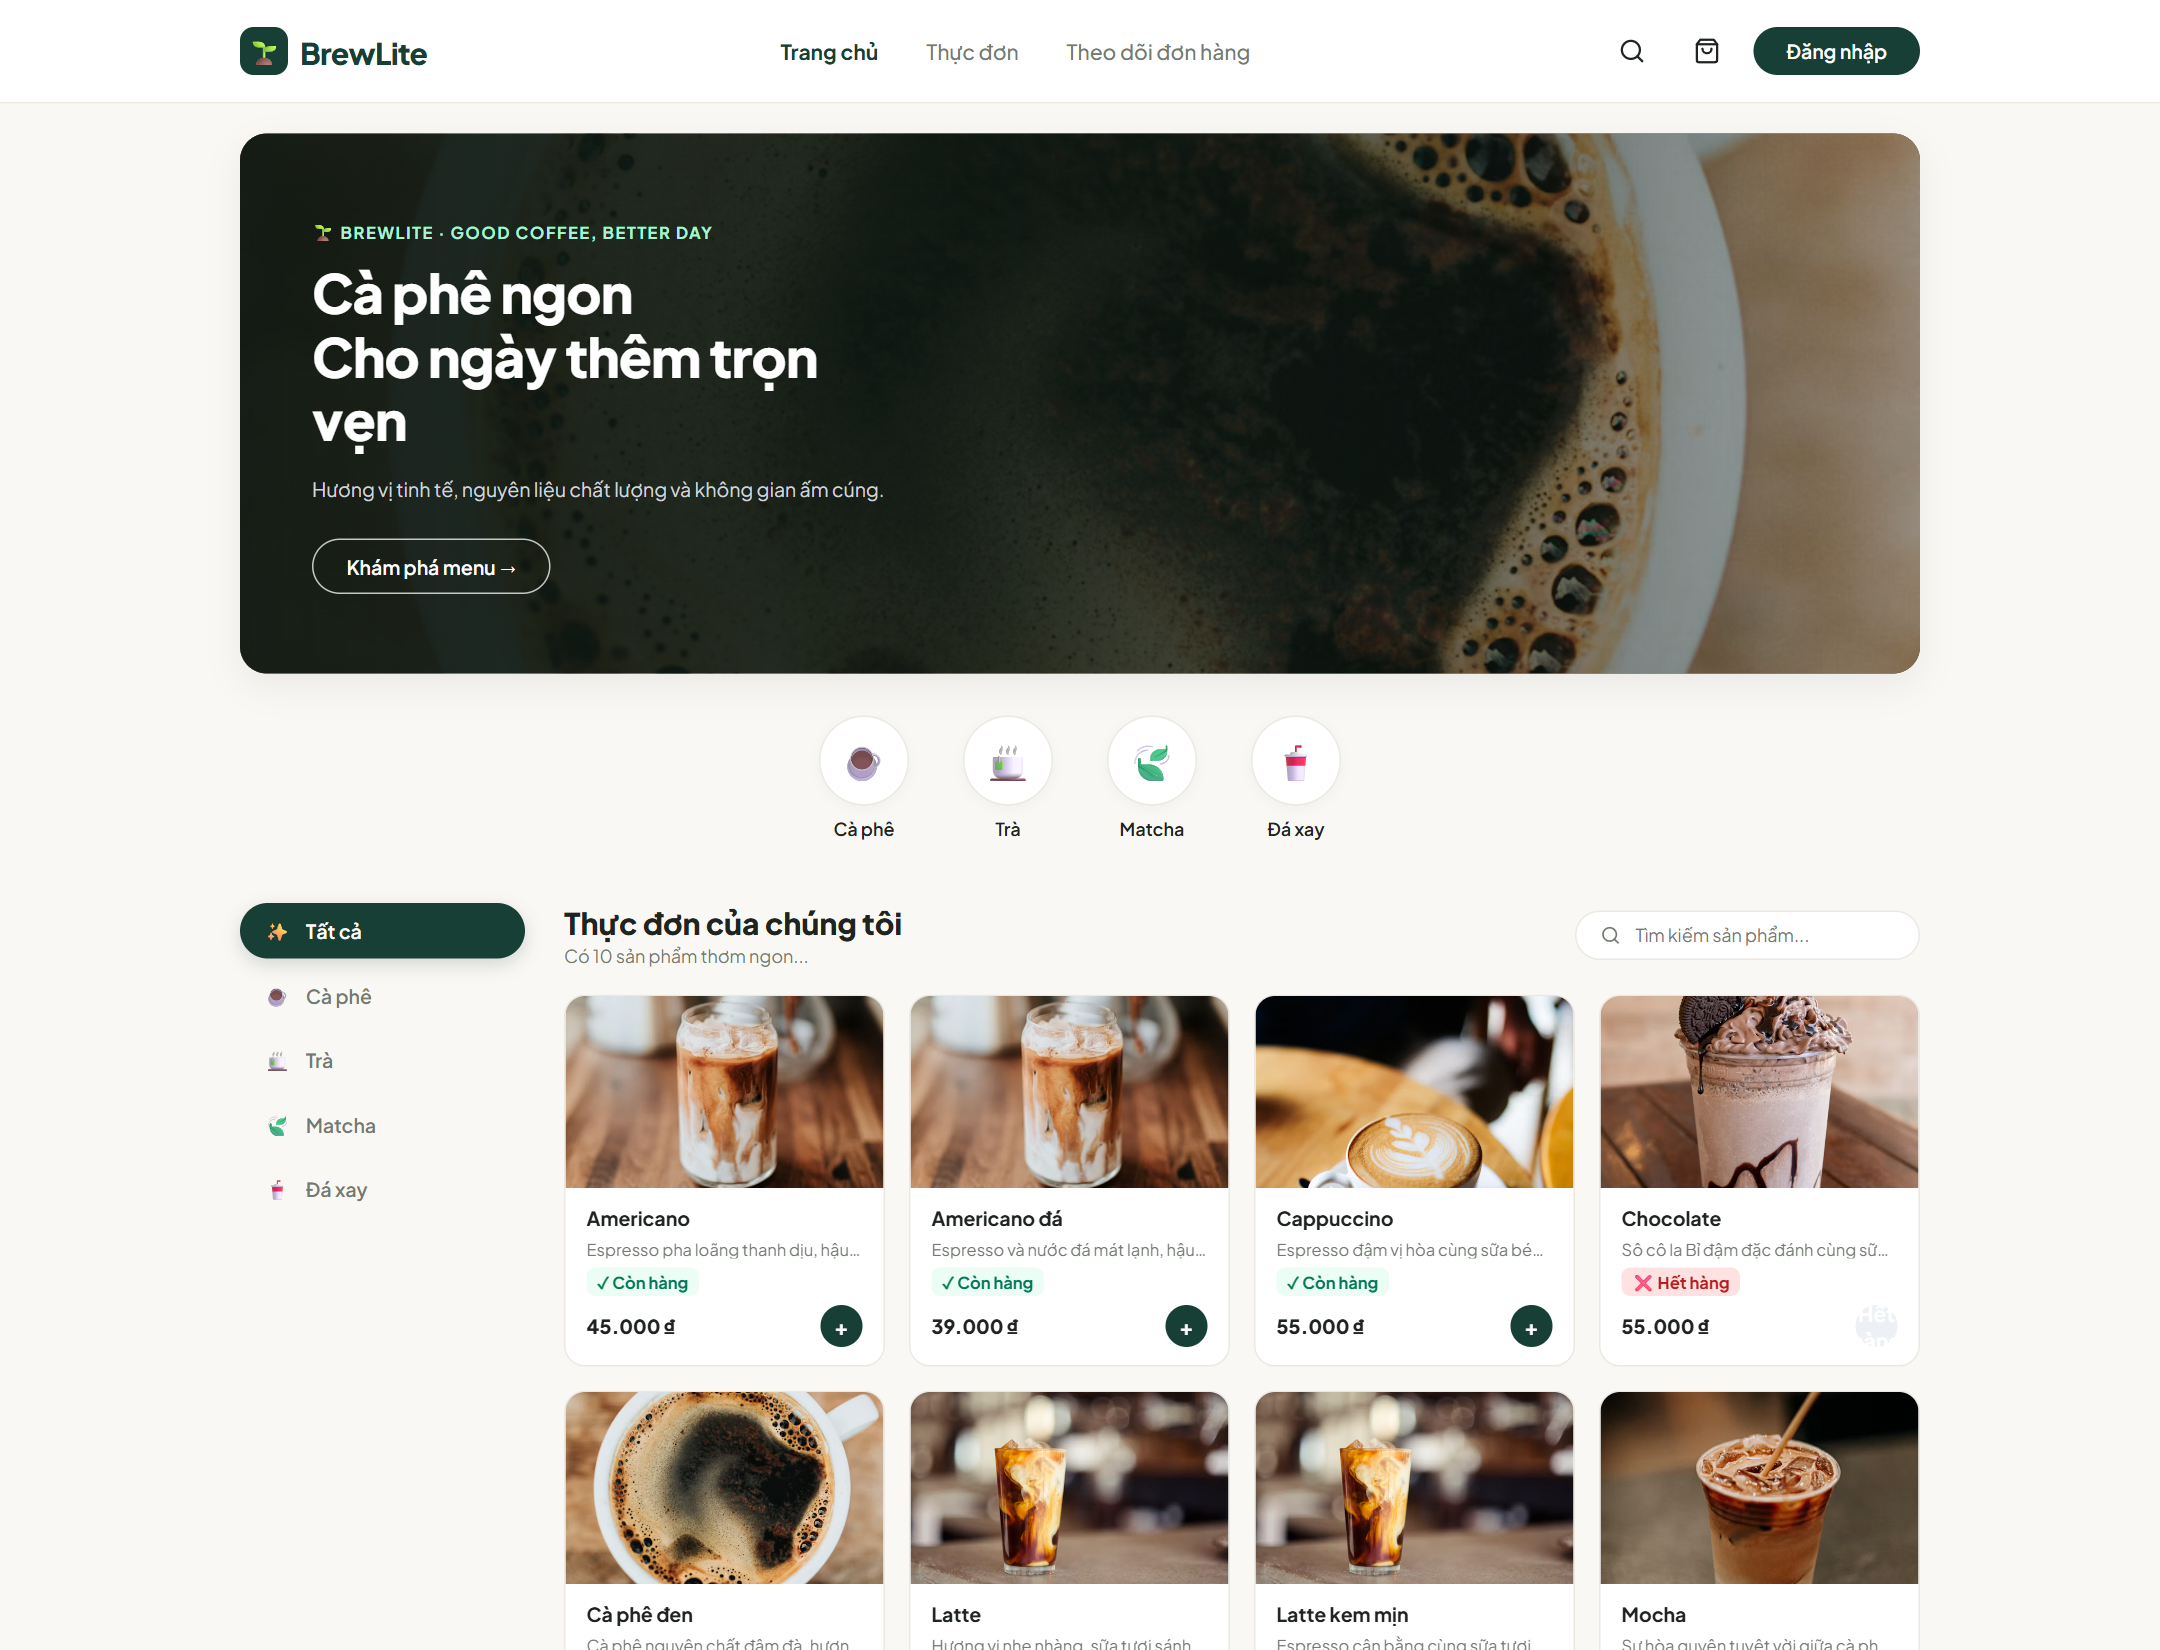
\includegraphics[width=\linewidth,height=0.55\textheight,keepaspectratio]{hinh/giao-dien-thuc-don.png}
\caption{Ảnh giao diện thực đơn chụp từ phiên bản chạy local.}
\label{fig:menu}
\end{figure}

\subsubsection{Xử lý trạng thái UI và dữ liệu}
Khi chưa có dữ liệu, UI thể hiện đang tải; danh sách rỗng có thông điệp riêng; lỗi API có nút thử lại. Dữ liệu mẫu được seed qua Prisma. Với lỗi thiếu nguyên liệu, thông báo khách hàng được rút gọn, không hiển thị tên và định lượng tồn kho nội bộ.

\subsubsection{Viết test cơ bản}
Unit test API sản phẩm kiểm tra món đang hoạt động, topping hợp lệ, trường hợp không có món và 404. Kiểm thử trình duyệt chặn phản hồi sản phẩm để xác minh empty/error và khả năng thử lại. Đây là kiểm thử chức năng, khác với ảnh chụp minh họa.

\subsection{Continuous Integration}
\subsubsection{Cấu hình pipeline CI}
\tep{.github/workflows/ci.yml} khai báo pipeline khi pull request/push và cho phép workflow khác gọi lại. Các bước chính: npm ci, sinh Prisma Client, lint, unit test, build, migration/seed database test, integration và Playwright E2E. PostgreSQL kiểm thử có tên database/credentials riêng, tách khỏi dữ liệu demo.

\begin{figure}[H]\centering
\begin{tikzpicture}[node distance=4mm]
\node[hop,text width=2.1cm] (a) {Cài đặt};
\node[hop,text width=1.8cm,right=of a] (b) {Lint};
\node[hop,text width=2.1cm,right=of b] (c) {Unit test};
\node[hop,text width=1.8cm,right=of c] (d) {Build};
\node[hop,text width=2.9cm,right=of d] (e) {Integration / E2E};
\draw[mui] (a)--(b);\draw[mui] (b)--(c);\draw[mui] (c)--(d);\draw[mui] (d)--(e);
\end{tikzpicture}
\caption{Các bước quality gate được khai báo trong CI.}
\end{figure}

\subsubsection{Khóa nhánh theo chất lượng code}
Điều kiện đề bài là không merge nếu lint/test/build thất bại. YAML không tự tạo branch protection; cần đặt required status checks/ruleset trên GitHub, yêu cầu review và lưu minh chứng. Chưa có đường dẫn hosted PR chạy thành công/thất bại hoặc ảnh cấu hình required checks trong gói hiện tại.

\clearpage
\section{Task 5 - Sprint 2, CI/CD và delivery}
\subsection{Hoàn thiện MVP}
\subsubsection{Chi tiết sản phẩm và tùy chọn}
Khách chọn size, topping và số lượng; API kiểm tra item và tính tổng theo dữ liệu chuẩn. Các tùy chọn đã chọn được lưu vào dòng đơn để không bị thay đổi theo giá thực đơn sau thời điểm đặt.

\subsubsection{Giỏ hàng và thanh toán}
Giỏ hỗ trợ cập nhật, xóa và kiểm tra khả năng đáp ứng. Sau khi đăng nhập, khách xác nhận tạo đơn rồi nhận URL VNPay Sandbox. UI giữ giỏ khi lỗi; trạng thái success trên URL không tự xóa giỏ hoặc xác nhận PAID. Chữ ký kiểm thử chỉ dùng ở môi trường test riêng.

Đơn 0đ có xử lý xác nhận riêng; không mô tả việc chuyển cổng như điều kiện bắt buộc cho tất cả các đơn. Thiếu nguyên liệu hiện thông điệp gọn cho khách; thông tin định lượng chi tiết vẫn phục vụ logic và vận hành nội bộ.

\subsubsection{Quản lý đơn hàng và lịch sử}
Quản trị hiển thị đủ đơn chờ thanh toán, thanh toán lỗi, đã thanh toán, đang pha, sẵn sàng, hoàn tất và đã hủy. READY được hiển thị là ``Sẵn sàng nhận''. Bộ lọc không có kết quả hiển thị thông báo, không để bảng trống không giải thích.

Nút ``Hủy đơn'' chỉ có trước pha chế: PENDING, PAYMENT\_FAILED hoặc PAID. Có bước xác nhận; từ PREPARING không có nút hủy. Đơn PAID bị hủy sử dụng luồng hoàn tiền của backend; thanh toán REFUND\_PENDING hiển thị ``Đã hủy · Chờ hoàn tiền''. Khi mất kết nối, UI không cập nhật thành công giả.

\begin{figure}[H]\centering
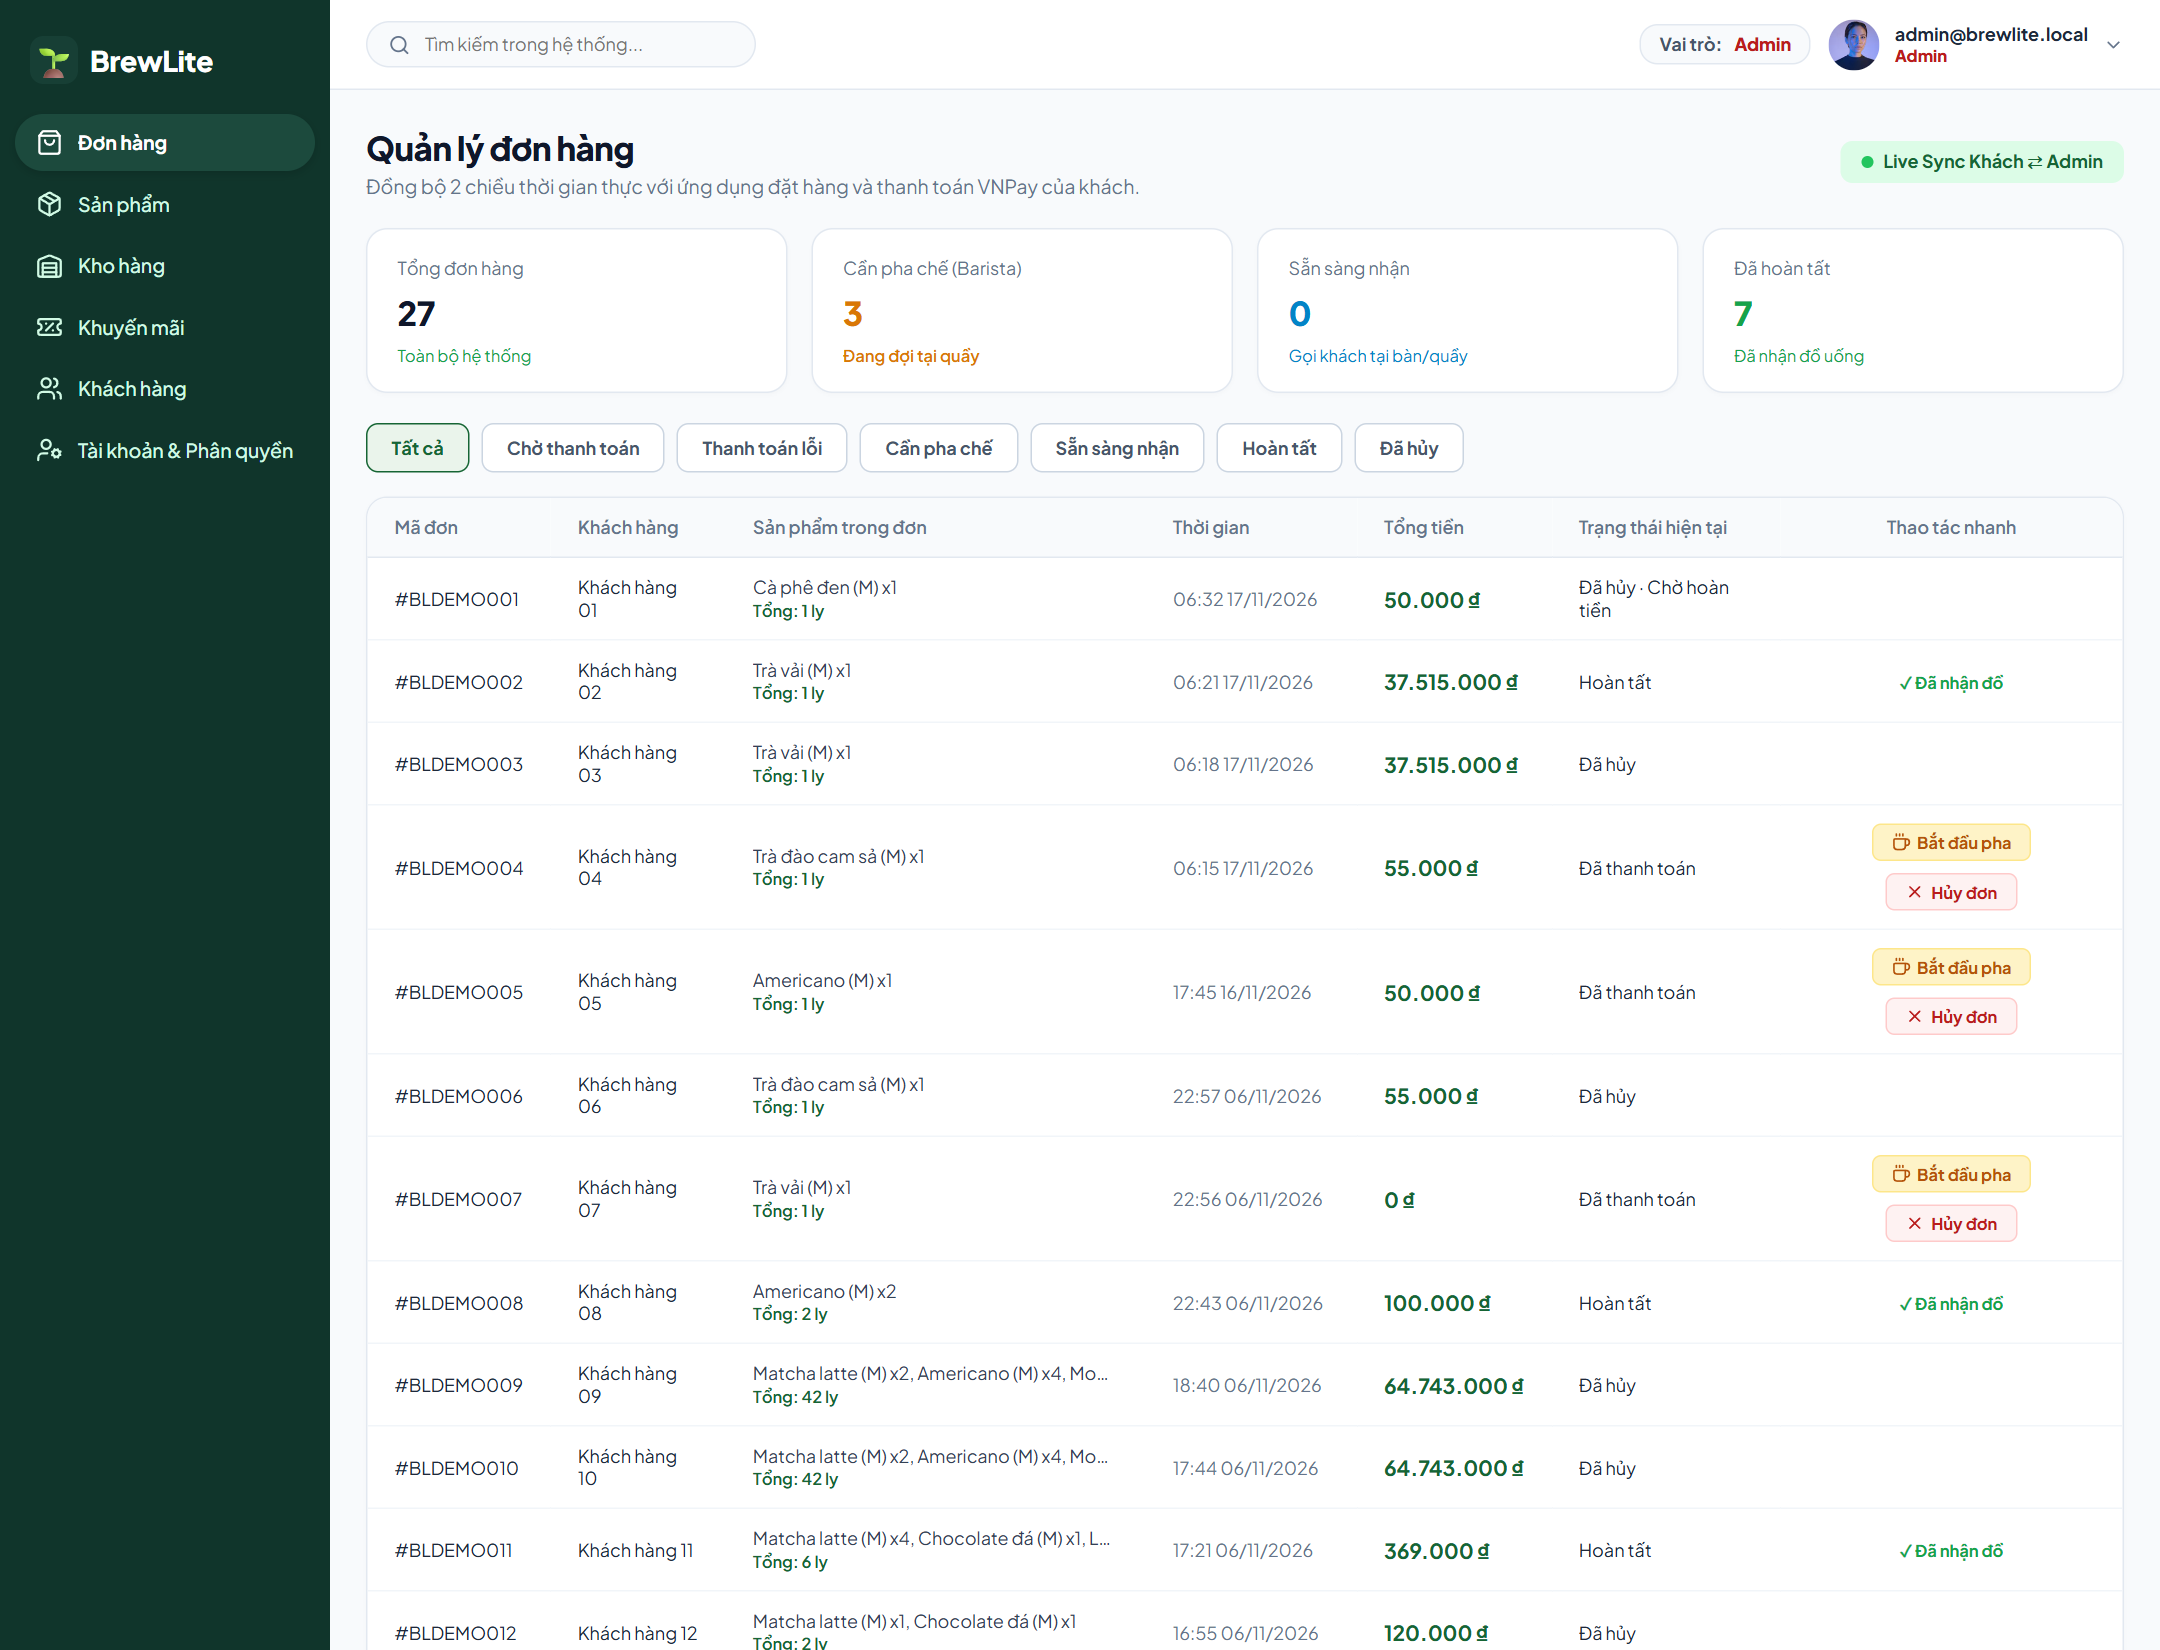
\includegraphics[width=\linewidth,height=0.60\textheight,keepaspectratio]{hinh/giao-dien-quan-tri.png}
\caption{Quản lý đơn hàng trên local; thông tin khách hàng đã được thay thế trên bản chụp phục vụ báo cáo.}
\label{fig:admin}
\end{figure}

\subsubsection{Validate dữ liệu}
Frontend kiểm tra input và trạng thái tương tác; backend kiểm tra DTO, JWT, quyền sở hữu, quyền vai trò, các tùy chọn và trạng thái chuyển tiếp. Không tin vào tổng tiền hoặc trạng thái do client tự gửi. Callback phải qua kiểm tra chữ ký/số tiền. Native dialog và thao tác UI không thay thế ràng buộc phía server.

\subsection{Tích hợp và kiểm thử}
\subsubsection{Unit và integration test}
Unit test tập trung vào nghiệp vụ giá, trạng thái, thanh toán, callback, retry và đọc cấu hình. Integration chạy HTTP thực với PostgreSQL riêng, kiểm tra JWT, tạo đơn, chữ ký sai, callback lặp, intent đồng thời, tranh ly cuối, hủy PAID và phân quyền.

\begin{table}[H]\centering\small
\begin{tabularx}{\textwidth}{P{4.0cm}P{2.4cm}Y}
\toprule\textbf{Nhóm kiểm tra local}&\textbf{Kết quả ghi nhận}&\textbf{Giới hạn kết luận}\\\midrule
Unit nghiệp vụ&46/46 đạt&Kết quả trước các chỉnh sửa UI thuần hiển thị sau đó.\\
Integration HTTP/PostgreSQL&18/18 đạt&Dùng database test riêng; không phải bằng chứng production.\\
E2E khách hàng và PWA&5/5 đạt&Luồng Sandbox dùng callback ký bằng khóa test riêng.\\
E2E quản trị sau thêm nút hủy&6/6 đạt&Bao gồm trạng thái, lỗi mạng, mobile và xác nhận hủy.\\
TypeScript, lint và Docker build&Đạt ở các lần kiểm tra tương ứng&Không thay thế hosted quality gate.\\
API thực đơn warm p95&44,6 ms / 30 request&Số đo local, không suy rộng cho tải production.\\
\bottomrule\end{tabularx}\caption{Kết quả local đã được ghi nhận trong quá trình kiểm tra dự án.}
\end{table}
Các nhóm E2E được kiểm tra ở các thời điểm riêng; bảng không khẳng định một lần chạy duy nhất có 11 ca sau mọi thay đổi. Cần lưu log/ảnh CI và chốt lại toàn bộ test trên commit nộp bài.

\subsubsection{End-to-end test}
Ca chính đi qua menu, đăng nhập, chọn món, giỏ hàng, yêu cầu thanh toán, callback test và xác nhận. Ca âm kiểm tra URL success giả, lỗi tạo liên kết, phản hồi menu rỗng/lỗi. Quản trị có test chỉ hiện nút hủy trước pha; từ chối xác nhận không gửi PATCH; đồng ý hủy cập nhật theo phản hồi server.

\subsubsection{Cấu hình vận hành tại local}
Compose local chạy web, API và PostgreSQL; database có healthcheck. API chạy migration và seed trước start. Cấu hình test dùng PostgreSQL cổng 55432, API 4100 và web 3100. Không chạy các test thay đổi kho/điểm trên dữ liệu demo hoặc production.

\begin{table}[H]\centering\small
\begin{tabularx}{\textwidth}{P{4.0cm}Y}
\toprule\textbf{Thành phần}&\textbf{Địa chỉ local}\\\midrule
Website&\url{http://localhost:3000}\\
Quản trị&\url{http://localhost:3000/admin}\\
API liveness&\url{http://localhost:4000/health}\\
Database readiness&\url{http://localhost:4000/health/ready}\\
PostgreSQL phát triển&localhost:5437 theo cấu hình hiện tại\\
\bottomrule\end{tabularx}\caption{Các địa chỉ local đã được kiểm tra; không phải URL production.}
\end{table}

\subsection{Continuous Delivery/Deployment}
\subsubsection{Hoàn thiện pipeline CD}
Workflow delivery chạy theo tag hoặc thủ công, gọi quality workflow, build image api/web từ các target trong root Dockerfile, gắn tag SHA và push GHCR. Job deploy chỉ được bật khi cấu hình ENABLE\_DEPLOY và secrets hợp lệ. Tệp script triển khai được chuyển lên VPS trước khi chạy.

\begin{figure}[H]\centering
\begin{tikzpicture}[x=1cm,y=1cm]
\node[tacvu] (a) at (0,0) {Push / tag};
\node[tacvu] (b) at (5,0) {Lint, test và build};
\node[tacvu] (c) at (10,0) {Build image theo SHA};
\node[tacvu] (d) at (10,-2) {Push GHCR};
\node[tacvu] (e) at (5,-2) {Deploy; migration an toàn};
\node[tacvu] (f) at (0,-2) {Smoke test HTTPS};
\node[tacvu] (g) at (0,-4) {Đạt: ghi release tag};
\node[tacvu] (h) at (5,-4) {Lỗi: dừng và rollback};
\draw[mui] (a)--(b);\draw[mui] (b)--(c);\draw[mui] (c)--(d);\draw[mui] (d)--(e);\draw[mui] (e)--(f);
\draw[mui] (f)--node[nhan,left]{Đạt}(g);\draw[mui] (f.south east)--node[nhan,above]{Thất bại}(h.north west);
\end{tikzpicture}

\caption{Chuỗi CD được cấu hình: quality gate, image, registry, triển khai và smoke test. Chưa có minh chứng hosted.}
\end{figure}

\subsubsection{Cơ chế an toàn}
\begin{enumerate}
\item Dùng image tag cố định và ghi nhận tag hiện tại/trước đó.
\item Pull image; chờ database healthy; chạy migration trước thay thế API/web.
\item Migration phải tương thích phiên bản trước, có kế hoạch backup trước khi phát hành.
\item Sau deploy, gọi readiness và web public; thất bại thì dừng pipeline và thử rollback image.
\item Rollback image không tự phục hồi database; migration phá vỡ tương thích cần phương án dữ liệu riêng.
\item Giữ PostgreSQL production trong mạng nội bộ; SSH known-hosts và secrets không được ghi vào log hay tài liệu công khai.
\end{enumerate}

\subsection{Triển khai và bàn giao}
\subsubsection{Môi trường production}
\begin{table}[H]\centering\small
\begin{tabularx}{\textwidth}{P{5.0cm}Y}
\toprule\textbf{Minh chứng cần nộp}&\textbf{Tình trạng}\\\midrule
URL frontend HTTPS công khai&\canbosung{URL đã truy cập được và ngày kiểm tra}\\
URL API và readiness HTTPS&\canbosung{URL và kết quả smoke test}\\
VPS/nền tảng và TLS/DNS&\canbosung{nhà cung cấp, cấu hình tương ứng sơ đồ}\\
PostgreSQL không public trực tiếp&Có cấu hình production; cần kiểm tra hạ tầng thực tế.\\
CI/CD hosted và branch protection&\canbosung{link PR, log pass/fail, required checks}\\
Release/tag và rollback&\canbosung{tag, release notes, log diễn tập}\\
\bottomrule\end{tabularx}\caption{Danh mục minh chứng production chưa được thay thế bằng kết quả local.}
\end{table}

\subsubsection{Tài liệu bàn giao và ma trận truy vết}
README chính chứa hướng dẫn thao tác. Phần 6 tổng hợp ma trận FR/NFR đến use-case, sơ đồ, code và test. Trước khi nộp phải đồng bộ nội dung này với các đường dẫn tài liệu bắt buộc của đề và với tên tệp thực tế sau đổi tên sang tiếng Việt.

Sprint Review cần ghi phiên bản demo, acceptance criteria đã đạt và góp ý; Retrospective cần ghi việc làm tốt, vấn đề và hành động cải tiến có người chịu trách nhiệm. Hiện chưa có ngày họp/biên bản thật, nên không tạo biên bản giả trong báo cáo.

\subsubsection{Đóng gói sản phẩm}
Gói bàn giao cần mã nguồn theo commit/tag xác định, báo cáo và sơ đồ nguồn/bản xuất, cấu hình mẫu, migration/seed, test, release notes, link video và hướng dẫn rollback. Không đóng gói node\_modules, dữ liệu database hoặc file secret thực tế.

\textbf{Kịch bản demo đề xuất:} mở menu; đăng nhập; chọn món/topping; kiểm tra tổng giỏ; thanh toán Sandbox; theo dõi trạng thái; tại quản trị bắt đầu pha, chuyển sẵn sàng và hoàn tất. Thêm một đơn độc lập để minh họa hủy trước pha và phân biệt chờ hoàn tiền. Không dùng test callback tự ký trên merchant thật để giả minh chứng ngân hàng.

\clearpage
\section{Ma trận truy vết và đánh giá hoàn thành}
\small
\begin{longtable}{P{1.35cm}P{2.0cm}P{3.0cm}P{4.0cm}P{3.8cm}}
\toprule\textbf{Yêu cầu}&\textbf{Use-case / story}&\textbf{Thiết kế}&\textbf{Code / API}&\textbf{Test / minh chứng}\\\midrule\endhead
FR-01&US-01 Xem món&Use-case tổng; class&GET /products; task-02-san-pham&san-pham.spec.ts; WEB-T01\\
FR-02&US-02 Tùy chọn&UC-01; class&GET /products/:id; tinh-gia-mon.ts&nghiep-vu.spec.ts; E2E chính\\
FR-03&US-03 Giỏ hàng&Activity; UC-01&/cart; task-05-gio-hang&INT-T01; E2E giỏ\\
FR-04&US-04 Xác thực&Sequence; UC-01&/auth/register, /auth/login; JWT guard&INT-T02; test phân quyền\\
FR-05&UC-01 Đặt đơn&Activity; sequence&POST /orders; task-06-don-hang&INT-T03; E2E chính\\
FR-06&UC-01 Trả tiền&Sequence; ADR-002&/payments/vnpay; retry-payment&Kiểm thử chữ ký/retry; IPN integration\\
FR-07&US-07 Theo dõi&Class; sequence&GET /orders/me; task-09-lich-su-don-hang&INT-T05; URL success giả\\
FR-08&US-08 Pha chế&Enum và quy tắc trạng thái&may-trang-thai-don-hang.ts; PATCH admin/orders/:id/status&nghiep-vu.spec.ts; 6 E2E quản trị\\
FR-09&UC-01 Gửi lặp&Sequence alt; khóa intent&POST /payments; Idempotency-Key&Integration intent đồng thời và IPN lặp\\
FR-10&UC-01 Ly cuối&Class nguyên liệu; sequence&task-10-ton-kho; Ingredient.version&Integration tranh ly cuối\\
FR-11&UC-01 Ưu đãi&Class; transaction&promotion, loyalty settlement&Unit giá/điểm; integration callback\\
FR-12&US-12 Nhân viên&Use-case actor; guard&task-10-quan-tri; bao-ve.guard.ts&403 cho khách; E2E quản trị\\
NFR-01&Xem món&Kiến trúc API&GET /products&PERF-T01; p95 local\\
NFR-02&Luồng bảo vệ&Sequence; ranh giới secret&JWT, DTO, bcrypt, chữ ký&INT-T02; unit chữ ký\\
NFR-03&Dùng trên mobile&Thiết kế UI; health&/health; /health/ready&Mobile 390 px; E2E lỗi mạng\\
NFR-04&Tái tạo&ADR-001; Docker&Compose, Dockerfile, Prisma&Migration/seed database test; Docker build\\
NFR-05&Phát hành&Deployment; pipeline&CI/delivery workflow; script deploy/rollback&Có cấu hình; minh chứng hosted còn thiếu\\
NFR-06&PWA&Kiến trúc web&manifest.ts; sw.js; offline.html&pwa.spec.ts; HTTPS production chưa chốt\\
\bottomrule
\end{longtable}
\normalsize
\subsection*{Kết luận về mức độ đáp ứng}
Sản phẩm có các thành phần và kiểm thử local cho luồng nghiệp vụ cốt lõi, đồng thời xử lý nhiều trường hợp ngoại lệ như callback lặp, tranh nguyên liệu và mất kết nối UI. Các Task 1--3 có nội dung mô tả trong báo cáo và nguồn sơ đồ đi kèm.

Tuy nhiên, chưa đủ cơ sở tuyên bố toàn bộ Assignment 2 đã được nghiệm thu: còn thiếu minh chứng lịch sử tuần tự, cấu hình bảo vệ nhánh/CI hosted, URL production hoạt động và các tạo phẩm Scrum/bàn giao. Khác biệt VNPay Sandbox so với thanh toán mô phỏng phải được nêu rõ với người chấm.

\clearpage
\appendix
\section{Hướng dẫn chạy và bàn giao}
\subsection{Chạy local}
Chạy trong thư mục gốc, mở Docker Desktop trước. Chỉ tạo .env từ mẫu nếu chưa có; điền merchant Sandbox ở máy của nhóm, không đưa vào báo cáo.
\begin{verbatim}
Copy-Item .env.example .env      # Chi khi chua co .env
docker compose up -d --build
docker compose ps
docker compose logs --tail 100 api web
\end{verbatim}
Lệnh \tep{docker compose down} giữ volume nếu không thêm \tep{-v}. Không xóa volume để giải quyết lỗi môi trường khi chưa có backup/ý định xóa dữ liệu.

\subsection{Kiểm thử và build}
\begin{verbatim}
npm ci
npm run db:generate
npm run lint
npm test
npm run build
docker compose -f docker-compose.test.yml up -d --wait
npm run test:setup
node tests/chay-voi-moi-truong-kiem-thu.cjs run start:prod -w apps/api
\end{verbatim}
Giữ terminal API test đang chạy; ở terminal khác:
\begin{verbatim}
node tests/chay-voi-moi-truong-kiem-thu.cjs run test:integration
npx playwright install chromium
node tests/chay-voi-moi-truong-kiem-thu.cjs run test:e2e
\end{verbatim}
Khi xong, dừng API test bằng Ctrl+C và dừng database test. Không dùng tên database production để chạy bộ integration.

\subsection{Deploy và rollback}
Trên VPS Linux đã cấu hình secrets, registry authentication, DNS và reverse proxy:
\begin{verbatim}
sh scripts/trien-khai.sh <commit-sha-da-push-image>
sh scripts/khoi-phuc-phien-ban.sh
\end{verbatim}
Database cần backup riêng. Việc gọi rollback không đồng nghĩa migration được hoàn nguyên.

\section{Phân công và kiểm tra trước khi nộp}
\subsection{Danh sách và đóng góp}
\begin{table}[H]\centering\small
\begin{tabularx}{\textwidth}{P{2.4cm}YcP{4.2cm}}
\toprule\textbf{MSSV}&\textbf{Thành viên}&\textbf{Tỷ lệ}&\textbf{Phần phụ trách}\\\midrule
3124410030&Võ Ngọc Chương&17\%&\canbosung{nhiệm vụ}\\
3120410101&Đỗ Xuân Quý Dương&17\%&\canbosung{nhiệm vụ}\\
3124560080&Nguyễn Thông Thái&15\%&\canbosung{nhiệm vụ}\\
3124410395&Trần Văn Minh Tuấn&17\%&\canbosung{nhiệm vụ}\\
3123560069&Nuyễn Thanh Quang&17\%&\canbosung{nhiệm vụ}\\
3124410130&Trần Nguyễn Thành Hưng&17\%&\canbosung{nhiệm vụ}\\
\midrule\multicolumn{2}{r}{\textbf{Tổng}}&100\%&\\\bottomrule
\end{tabularx}\caption{Tỷ lệ theo danh sách nhóm cung cấp; nhiệm vụ chi tiết chưa được cung cấp.}
\end{table}

\subsection{Checklist minh chứng}
\begin{itemize}[label=$\square$]
\item Điền thông tin bìa; xác nhận chính tả họ tên và phần phụ trách của từng thành viên.
\item Xác nhận quyền truy cập repository cho giảng viên và commit/tag nộp bài.
\item Đồng bộ SRS, use-case, activity, sequence, class và deployment với phiên bản code.
\item Khôi phục/tạo đúng các đường dẫn tài liệu bắt buộc của đề, gồm ma trận truy vết và deployment.
\item Chốt test trên commit cuối; lưu log pipeline thành công và một lần phát hiện lỗi.
\item Cấu hình required checks và minh chứng review/PR theo lịch sử thật.
\item Bổ sung URL HTTPS frontend/API, health và kiểm tra database không public.
\item Bổ sung release notes, video demo, Sprint Review và Retrospective thật.
\item Kiểm tra không có secret trong mã, hình, log, gói ZIP và báo cáo.
\end{itemize}

\section{Nguồn đối chiếu và cấu trúc gói LaTeX}
\begin{enumerate}
\item Đề bài \textit{Assignment2-BrewLite.pdf}, phiên bản 1.0, 8 trang.
\item \tep{docs/requirements/}: context-and-scope, SRS và use-case checkout.
\item \tep{docs/architecture/tong-quan.md} và các ADR trong cùng thư mục.
\item Mã nguồn \tep{apps/web}, \tep{apps/api}, Prisma schema/migration và cấu hình Docker/CI/CD.
\item Các ca unit, integration và E2E trong kho mã nguồn; kết quả local đã ghi nhận trong quá trình kiểm tra.
\end{enumerate}
Các sơ đồ TikZ của báo cáo nằm trong \tep{so-do/*.tex}, được biên dịch trực tiếp thành hình vector. Nguồn Mermaid hiện có của dự án cũng được giữ trong thư mục so-do để đối chiếu. Ảnh giao diện nằm trong hinh; không cần đường dẫn tuyệt đối trên máy người soạn.

Hướng dẫn biên dịch XeLaTeX/Tectonic và sửa thông tin bìa: \tep{huong-dan-bien-dich.txt}.
\end{document}
